\section{Thực nghiệm \& Kết luận}

% ==================== EXPERIMENTAL RESULTS ====================
\begin{frame}{Validation thực nghiệm (Paper Figure 5)}
  \textbf{Setup:}
  \begin{itemize}
    \item Mạng 2 lớp, 50,000 hidden units
    \item Full-batch gradient descent
    \item Bit length $\ell$ từ 2 đến 30
  \end{itemize}

  \vspace{0.3cm}
  \textbf{Kết quả:} Ensemble complexity tăng theo $O(\ell^2 \log \ell)$ như lý thuyết dự đoán.
\end{frame}

\begin{frame}{Biểu đồ minh chứng}
\centering
\resizebox{0.85\textwidth}{!}{
  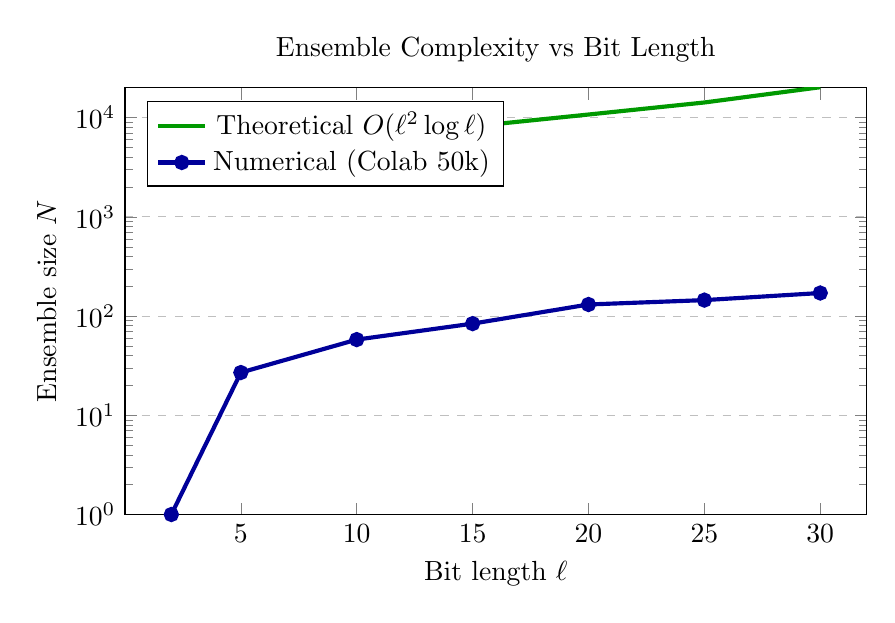
\begin{tikzpicture}
    \begin{semilogyaxis}[
        title={Ensemble Complexity vs Bit Length},
        xlabel={Bit length $\ell$},
        ylabel={Ensemble size $N$},
        xmin=0, xmax=32, ymin=1, ymax=20000,
        xtick={5,10,15,20,25,30},
        legend pos=north west,
        ymajorgrids=true, grid style=dashed,
        width=11cm, height=7cm,
    ]
    \addplot[color=green!60!black, line width=1.5pt]
    coordinates {(2.0,5013.9) (5,5195.7) (10,6400.9) (15,8174.6) (20,10772.9) (25,14246.0) (30,20305.4)};
    \addlegendentry{Theoretical $O(\ell^2 \log \ell)$}
    
    \addplot[color=blue!60!black, mark=*, line width=1.5pt]
    coordinates {(2,1) (5,27) (10,58) (15,84) (20,131) (25,145) (30,171)};
    \addlegendentry{Numerical (Colab 50k)}
    \end{semilogyaxis}
  \end{tikzpicture}
}
\end{frame}

% ==================== KẾT LUẬN ====================
\begin{frame}{Kết luận}
  \textbf{Điều bài báo đã chứng minh:}
  \begin{itemize}
    \item Mạng 2 lớp ($n_h \to \infty$) học \textbf{chính xác} lệnh thuật toán nhị phân.
    \item Chỉ cần $O(b)$ training samples (logarithmic).
    \item Ensemble: $N \in O(\ell^2 \log \ell)$.
  \end{itemize}

  \vspace{0.3cm}
  \textbf{Ý nghĩa:}
  \begin{itemize}
    \item Kết quả NTK-based đầu tiên cho exact learnability.
    \item SBN Turing-complete $\Rightarrow$ mở rộng cho mọi hàm tính được.
  \end{itemize}
\end{frame}

\begin{frame}{Hạn chế và hướng phát triển}
  \textbf{Hạn chế:}
  \begin{itemize}
    \item Giả định: Data \textbf{orthogonality}, truy cập instruction.
    \item \textbf{Bounded memory}: Cần retrain nếu đổi input size.
    \item Chưa hỗ trợ: Kiến trúc variable-length (RNN, Transformer).
  \end{itemize}

  \vspace{0.3cm}
  \textbf{Hướng phát triển:}
  \begin{itemize}
    \item Nghiên cứu \textbf{correlated data}.
    \item GNN (bounded degree) để đạt \textbf{length generalization}.
    \item Mở rộng lý thuyết: Transformer, kiến trúc mới.
  \end{itemize}
\end{frame}

% ===== SLIDE KẾT THÚC =====
\begin{frame}{}
  \centering
  \vfill
  {\Huge \textbf{Cảm ơn!}}\\[0.5cm]
  {\Large Q\&A}
  \vfill
\end{frame}
